\chapter{Arhitektura i dizajn sustava}
		


	
	Arhitektura aplikacije može se podijeliti na 3 djela. 
	
	\begin{packed_item}
		\item web poslužitelj
		
		\item web preglednik
		
		\item baza podataka
	
	\end{packed_item}
	
	\underbar{Web preglednik} je program koji korisniku omogućuje pristup web stranicama te multimedijskom sadržaju na njima. Web preglednik omogućuje korisniku pristup web poslužitelju putem HTTPS (eng. \textit{Hypertext Transfer Protokol Secure}) protokola te interpretira sadržaj kojeg je poslao Web poslužitelj u ljudski razumljiv oblik.
	
	\underbar{Web poslužitelj} je program koji prima i odgovara na korisnikove HTTPS zahtjeve. Web poslužitelj pokreće aplikaciju te korisniku šalje potrebne podatke kako bi korisnikov web preglednik mogao generirati frotnend aplikacije. Frontend predstavlja korisničko sučelje te je pisan u HTML-u, CSS-u i JavaScriptu uz pomoć React framework-a. Web poslužitelj je pisan u programskom jeziku Java i Spring Boot frameworku. Web poslužitelj komunicira sa bazom podataka te šalje podatke iz nje korisniku u prikladnom obliku.
	
	\underbar{Baza podataka} implementirana je putem PostgresSQL-a. Sadrži podatke potrebne za funkcioniranje aplikacije te njihove međusobne odnose. 

	
		

	
				
		\section{Baza podataka}
			
		
			
		Baza podataka za web aplikaciju koristi relacijski model podataka. Kao RDBMS (Relational Database Management System) koristi se PostgreSQL verzija 15.0. Koristeći ERDPlus, stvaramo ER dijagram baze podataka u kojem navodimo sve entitete, njihove atribute te međusobne veze. Daljnje tipove podataka, primarne, strane i alternativne ključeve navodimo u relacijskoj shemi baze podataka.
		
			
			\subsection{Opis tablica}
		
				\begin{longtblr}[
					label=none,
					entry=none
					]{
						width = \textwidth,
						colspec={|X[6,l]|X[6, l]|X[20, l]|}, 
						rowhead = 1,
					} %definicija širine tablice, širine stupaca, poravnanje i broja redaka naslova tablice
					\hline \SetCell[c=3]{c}{\textbf{User}}	 \\ \hline[3pt]
					\SetCell{LightGreen}id & VARCHAR(10)	&  	Jedinstveni identifikator svakog zaposlenika  	\\ \hline
					name	& CHAR(30) &   Ime korisnika	\\ \hline
                    surname & CHAR(30) &   Prezime korisnika    \\ \hline 
					function & CHAR(10) &   Funkcija svakog zaposlenika (limitirano na Zaposlenik, Revizor, Računovođa i Direktor)   \\ \hline 
					password & VARCHAR(30)	&  	Korisnikova lozinka	\\ \hline 
					email & VARCHAR(50)   &   E-mail korisnika \\ \hline
				\end{longtblr}
				
				\begin{longtblr}[
					label=none,
					entry=none
					]{
						width = \textwidth,
						colspec={|X[6,l]|X[6, l]|X[20, l]|}, 
						rowhead = 1,
					}
					\hline \SetCell[c=3]{c}{\textbf{Photos}}	 \\ \hline[3pt]
					\SetCell{LightBlue} id	& VARCHAR(10)   &   Jedinstveni identifikator zaposlenika izveden iz tablice RegisteredUser	\\ \hline
                    \SetCell{LightGreen} photoID  & VARCHAR(10)   &   Jedinstveni identifikator fotografije \\ \hline
                    url   & VARCHAR(255)   &  URL fotografije \\ \hline
                    imageName   & VARCHAR(10)  &  Ime prenesene fotografije \\ \hline
                    uploadTime  & TIMESTAMP  &  Datum i vrijeme prijenosa fotografije \\ \hline
				\end{longtblr}

                \begin{longtblr}[
					label=none,
					entry=none
					]{
						width = \textwidth,
						colspec={|X[6,l]|X[6, l]|X[20, l]|}, 
						rowhead = 1,
					}
					\hline \SetCell[c=3]{c}{\textbf{Document}}	 \\ \hline[3pt]
                    \SetCell{LightBlue} id  &  VARCHAR(10)  &  Jedinstveni identifikator zaposlenika izveden iz tablice RegisteredUser	\\ \hline
                    \SetCell{LightGreen} documentID  &  VARCHAR(10)  &  Jedinstveni identifikator prenesenog dokumenta \\ \hline
                    verifierID  &  VARCHAR(10)  &  Jedinstveni identifikator zaposlenika koji je potvrdio dokument \\ \hline
                    correct  &  BOOLEAN  &  Potvrda ukoliko je rezultantni dokument ispravno skeniran \\ \hline
                    documentType  &  VARCHAR(20)  &  Tip dokumenta (limitirano na Račun, Ponuda i Interni dokument) \\ \hline
                    signed  &  BOOLEAN  &  Potvrda ukoliko je rezultantni dokument potpisan od strane direktora \\ \hline
                    verified  &  BOOLEAN  &  Potvrda ukoliko je rezultantni dokument potpisan od strane računovođe \\ \hline
                    superVerified  &  BOOLEAN  &  Potvrda ukoliko je rezultantni dokument potpisan od strane nadležne osobe \\ \hline
                \end{longtblr}

                \begin{longtblr}[
					label=none,
					entry=none
					]{
						width = \textwidth,
						colspec={|X[6,l]|X[6, l]|X[20, l]|}, 
						rowhead = 1,
					}
					\hline \SetCell[c=3]{c}{\textbf{ArchiveReciept}}	 \\ \hline[3pt]
                    \SetCell{LightBlue} documentID  &  VARCHAR(10)  &  Jedinstveni identifikator dokumenta koji se arhivira \\ \hline
                    \SetCell{LightGreen} arcRecID  &  VARCHAR(10)  &  Jedinstveni identifikator dokumenta koji se nalazi u arhivi računa \\ \hline
                    clientName  &  VARCHAR(50)  &  Ime klijenta \\ \hline
                    totalPrice  &  FLOAT  &  Ukupna cijena \\ \hline
                \end{longtblr}

                \begin{longtblr}[
					label=none,
					entry=none
					]{
						width = \textwidth,
						colspec={|X[6,l]|X[6, l]|X[20, l]|}, 
						rowhead = 1,
					}
					\hline \SetCell[c=3]{c}{\textbf{ArchiveOffer}}	 \\ \hline[3pt]
                    \SetCell{LightBlue} documentID  &  VARCHAR(10)  &  Jedinstveni identifikator dokumenta koji se arhivira \\ \hline
                    \SetCell{LightGreen} arcOfferID  &  VARCHAR(10)  &  Jedinstveni identifikator dokumenta koji se nalazi u arhivi ponuda \\ \hline
                    totalPrice  &  FLOAT  &  Ukupna cijena \\ \hline
                \end{longtblr}

                \begin{longtblr}[
					label=none,
					entry=none
					]{
						width = \textwidth,
						colspec={|X[6,l]|X[6, l]|X[20, l]|}, 
						rowhead = 1,
					}
					\hline \SetCell[c=3]{c}{\textbf{ArchiveInternalDoc}}	 \\ \hline[3pt]
                    \SetCell{LightBlue} documentID  &  VARCHAR(10)  &  Jedinstveni identifikator dokumenta koji se arhivira \\ \hline
                    \SetCell{LightGreen} archIntDocID  &  VARCHAR(10)  &  Jedinstveni identifikator dokumenta koji se nalazi u arhivi internih dokumenata \\ \hline
                    text  &  TEXT  &  Tekst arhiviranog internog dokumenta  \\ \hline
                \end{longtblr}

                \begin{longtblr}[
					label=none,
					entry=none
					]{
						width = \textwidth,
						colspec={|X[6,l]|X[6, l]|X[20, l]|}, 
						rowhead = 1,
					}
					\hline \SetCell[c=3]{c}{\textbf{Articles}}	 \\ \hline[3pt]
                    \SetCell{LightBlue} arcRecID  &  VARCHAR(10)  &  Jedinstveni identifikator dokumenta koji se nalazi u arhivi računa izveden iz tablice ArchiveReciept \\ \hline
                    \SetCell{LightBlue} arcOfferID  &  VARCHAR(10)  &  Jedinstveni identifikator dokumenta koji se nalazi u arhivi ponuda izveden iz tablice ArchiveOffer \\ \hline
                    articleName  &  VARCHAR(50)  &  Ime artikla \\ \hline
                    price  &  FLOAT  &  Cijena artikla  \\ \hline
                \end{longtblr}    

			\subsection{Dijagram baze podataka}
				
				\begin{figure}[H]
					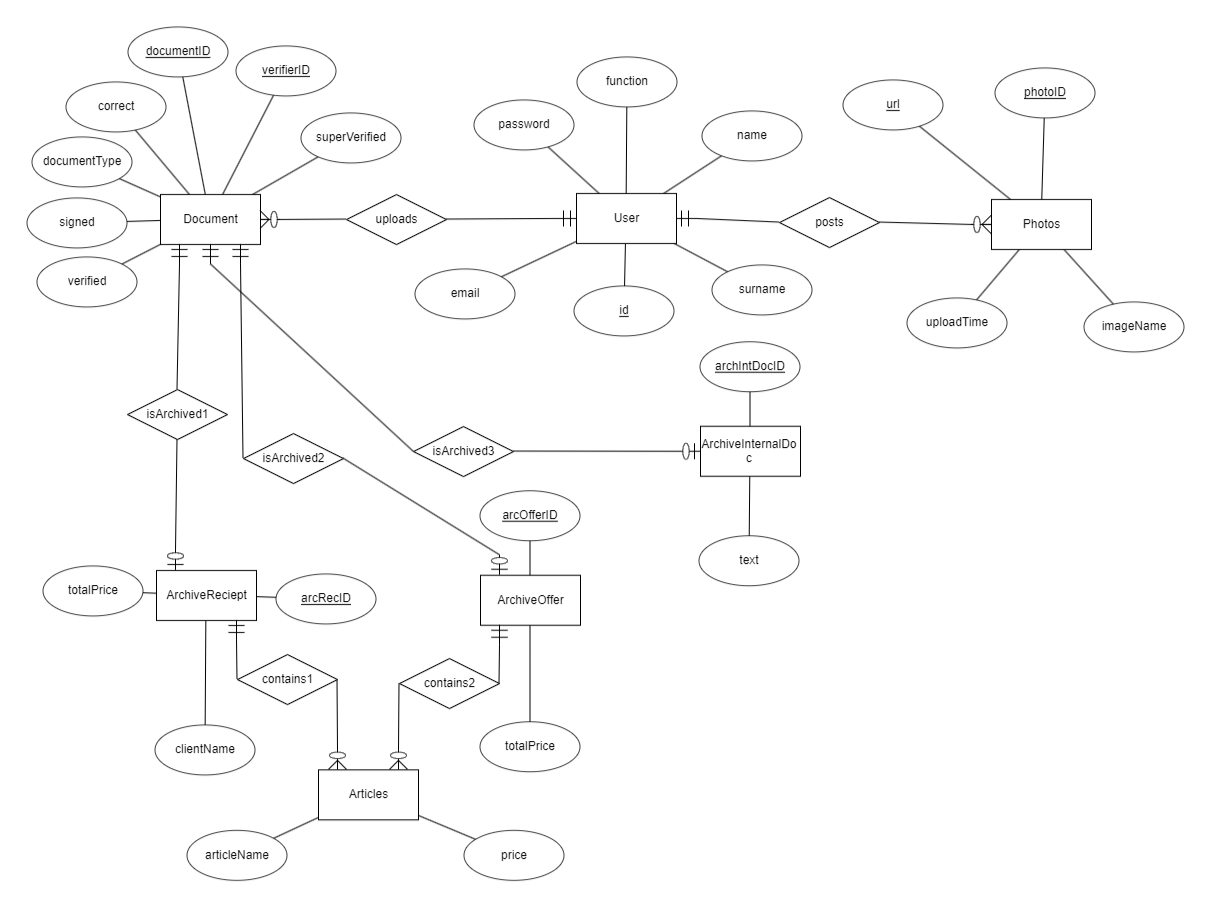
\includegraphics[scale=0.6]{slike/kompletici_v2_ER.PNG} %veličina slike u odnosu na originalnu datoteku i pozicija slike
					\centering
					\caption{ER dijagram baze podataka}
					\label{fig:promjene}
				\end{figure}
				
					\begin{figure}[H]
					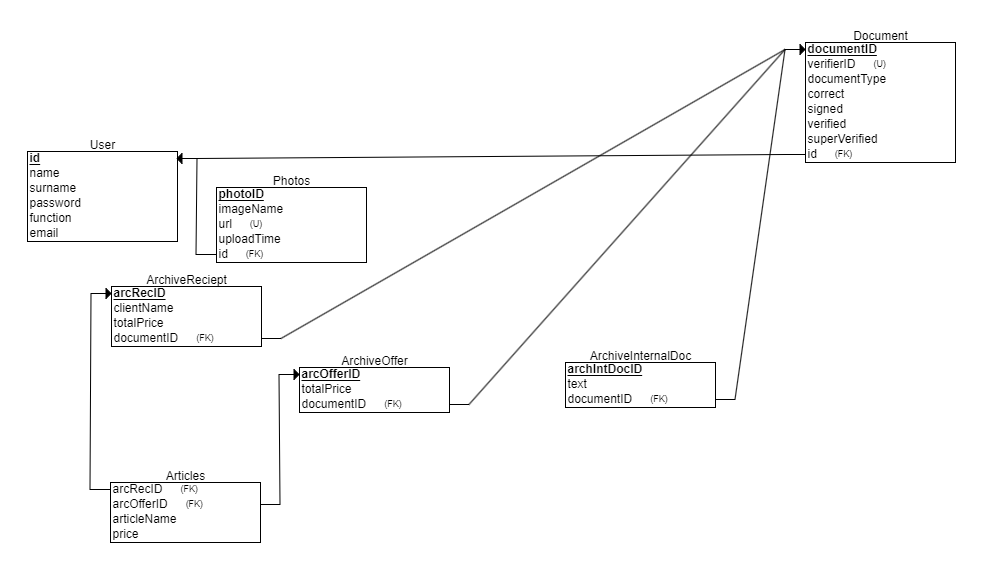
\includegraphics[scale=0.5]{slike/kompletici_v2_REL.PNG} %veličina slike u odnosu na originalnu datoteku i pozicija slike
					\centering
					\caption{REL dijagram baze podataka}
					\label{fig:promjene}
				\end{figure}
				
				
			
			\eject
			
			
		\section{Dijagram razreda}
		
			\begin{figure}[H]
				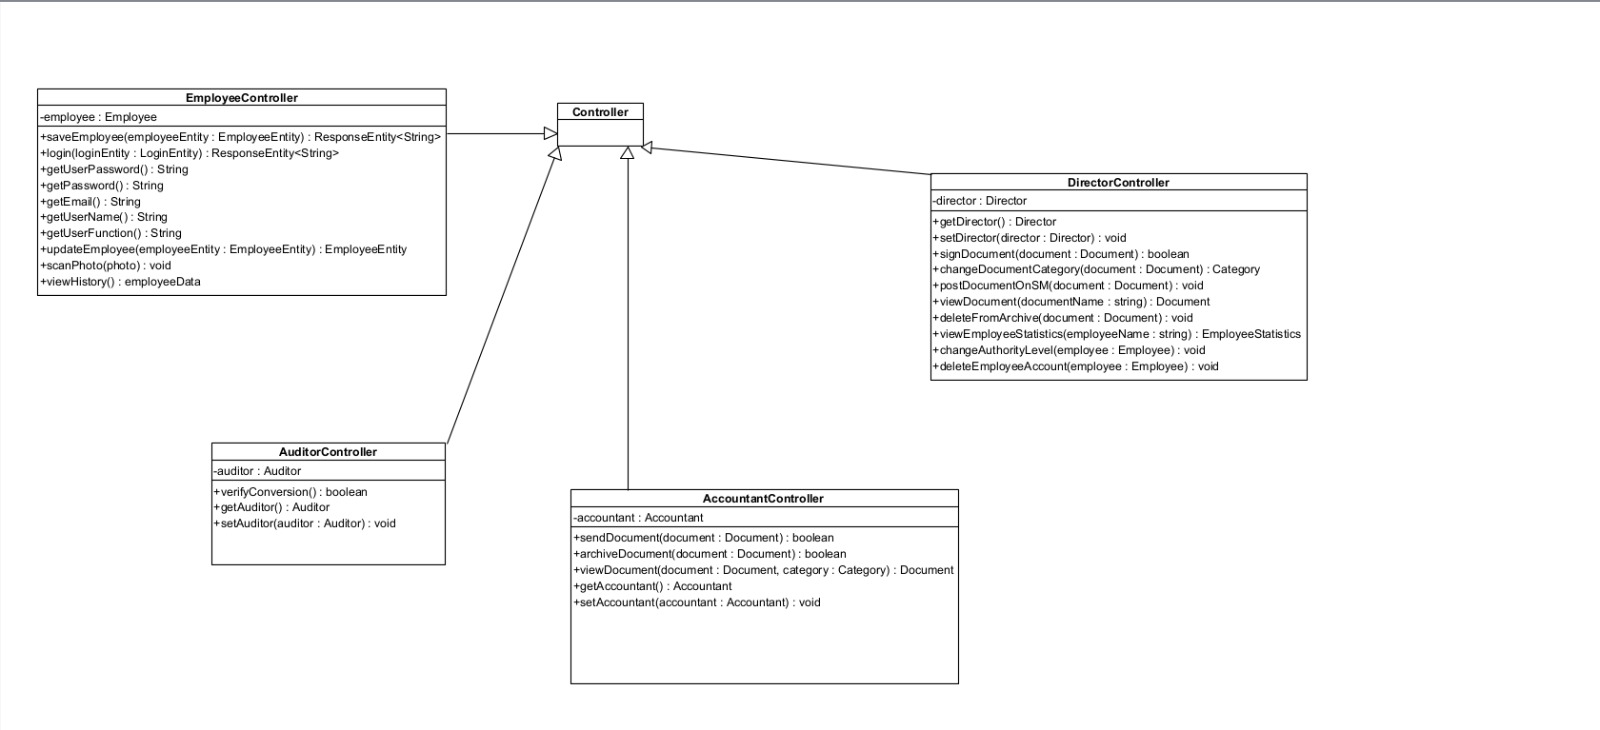
\includegraphics[scale=0.5]{slike/dijagram_razred1.jpeg} %veličina slike u odnosu na originalnu datoteku i pozicija slike
				\centering
				\caption{Dijagram razreda 1}
				\label{fig:promjene}
			\end{figure}
			
			\begin{figure}[H]
				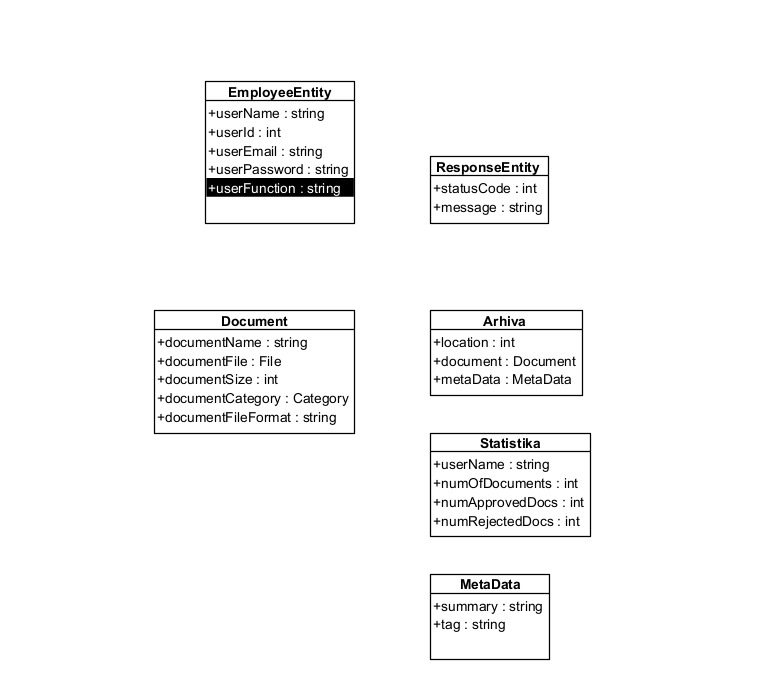
\includegraphics[scale=0.5]{slike/dijagram_razred2.jpeg} %veličina slike u odnosu na originalnu datoteku i pozicija slike
				\centering
				\caption{Dijagram razreda 2}
				\label{fig:promjene}
			\end{figure}
			
			
			
			\eject
		
		\iffalse
		\section{Dijagram stanja}
			
			
			\textbf{\textit{dio 2. revizije}}\\
			
			\textit{Potrebno je priložiti dijagram stanja i opisati ga. Dovoljan je jedan dijagram stanja koji prikazuje \textbf{značajan dio funkcionalnosti} sustava. Na primjer, stanja korisničkog sučelja i tijek korištenja neke ključne funkcionalnosti jesu značajan dio sustava, a registracija i prijava nisu. }
			
			
			\eject 
		
		\section{Dijagram aktivnosti}
			
			\textbf{\textit{dio 2. revizije}}\\
			
			 \textit{Potrebno je priložiti dijagram aktivnosti s pripadajućim opisom. Dijagram aktivnosti treba prikazivati značajan dio sustava.}
			
			\eject
		\section{Dijagram komponenti}
		
			\textbf{\textit{dio 2. revizije}}\\
		
			 \textit{Potrebno je priložiti dijagram komponenti s pripadajućim opisom. Dijagram komponenti treba prikazivati strukturu cijele aplikacije.}
		\fi